\chapter{Deep Leaning}

% Fazer um resumo

Um dos clássicos problemas na área
de classificação de imagens era o
reconhecimento de dígitos
escritos à mão. 
A dificuldade nesse tipo de problema
vinha pela grande variação de forma
e posição dos números, tornando 
os modelos muito complexos e pouco
precisos. O desenvolvimento
recente na área de Machine Learning
permitiu a criação de modelos
simples capazes de aprender com
os dados e fazer generalizações
precisas, em alguns casos
superando a percepção humana.

Neste capítulo serão apresentadas
técnicas que usam Redes Neurais,
como elas foram desenvolvendo
ao longo dos anos, e como podemos
aplicá-las na Síntese de Textura.


%\cite{Li2021}

\section{Aprendizado de Representação}
%19h


% Hierarquia de representações
No processo de análise de imagens,
precisamos criar representações
que melhor explicam seu conteúdo.
Essas representações podem ser organizadas
hierarquicamente, onde
a primeira identifica
arestas, a segunda indica cantos, etc.
Ao descer no nível das representações
queremos ter uma melhor informação
semântica da imagem.


Para um problema de classificação de imagens,
é preciso saber quais informações são 
úteis para obter uma melhor 
representação de seu conteúdo. 
Uma representação boa esconde informações
redundantes e realçar fatores que 
melhor explicam a imagem.
Bengio, Courville e Vincent
\cite{Bengio2014} falam do importante
papel que a aprendizagem
de representações tem em Machine Learning.
Um algoritmo que aprendesse tais representações
eliminaria o trabalho de desenvolvê-las,
o que tornaria mais rápido a criação de aplicações.


\section{Redes neurais}
%20h

% Definir o que é uma rede neural


Redes Neurais são um tipo 
de modelo de Machine Learning inspirado
em redes de neurônios naturais e como
eles se comunicam. Elas podem ser
representadas por um grafo, onde
cada nó representa um valor e cada aresta
representa uma dependência. Essas
redes podem ter vários formatos
dependendo do tipo de aplicação.

Um exemplo comum de Rede Neural é o Multi Layer
Perceptron. Nesse modelo, a rede é dividida
em camadas de diferentes tamanhos, e o dado
flui da camada de entrada até a saída,
que pode representar uma classificação
da entrada ou uma função geral.

% Imagem MLP

\begin{figure}[!ht]
	\centering
	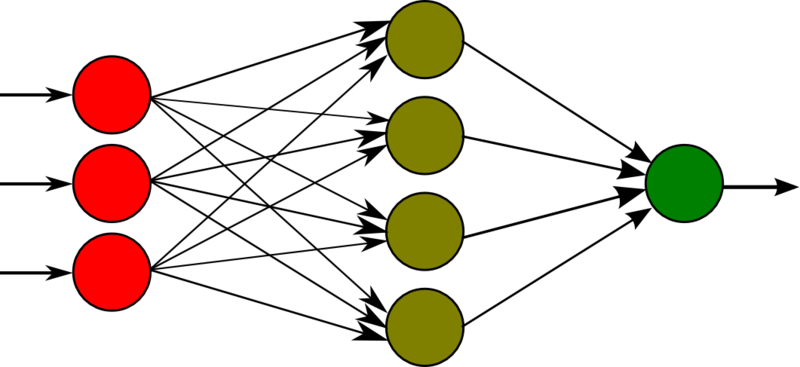
\includegraphics[width=\linewidth*2/3]{files/assets/deeplearning/mlp.png}
	\caption{Rede Multi Layer Perceptron. Cada camada da
	rede atua como uma representação do dado de entrada, que
	é usada para calcular a próxima camada.}
	\label{img:preview}
\end{figure}


Cada camada da rede tem como parâmetros os offsets 
$\mathbf{b}_m$ e uma matriz de pesos $\mathbf{W}_{m\times n}$.
Assim, a transformação da entrada $\mathbf{x}_n$ na saída
$\mathbf{y}_m$ pode ser representada com a seguinte operação:
\begin{equation}
	\mathbf{y} = 
	\varphi\left( \mathbf{W}\mathbf{x} + \mathbf{b} \right),
\end{equation}
onde $\varphi$ é uma função não linear, comummente chamada
de ``função de ativação''. A função não linear
mais comummente usada é a ReLU, que trunca valores
negativos no $0$.

\begin{figure}[!ht]
	\centering
	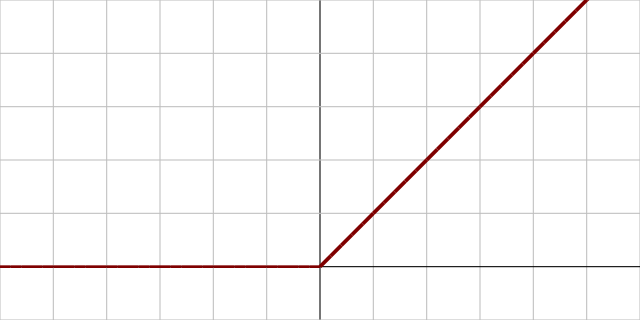
\includegraphics[width=\linewidth*2/3]{files/assets/deeplearning/relu.png}
	\caption{Função ReLU. O seu bico não diferenciável
	facilita a distorcer o espaço de entrada.}
	\label{img:preview}
\end{figure}

%Os parâmetros são tais que minimizam o erro 
%da saída. Essa minimização pode ser feita
%calculando o gradiente 
%\begin{equation}
%	\mathbf{y'} = 
%	\mathbf{W}\varphi'\left( \mathbf{W}\mathbf{x} + \mathbf{b} \right),
%\end{equation}

Os parâmetros são calculados minimizando
uma função de erro na saída. Essa minimização
é feita usando o gradiente dos parâmetros
em relação à função de perda. Como a derivada
de todas as funções aplicadas é conhecida,
o gradiente pode ser calculado computacionalmente
utilizando ``backpropagation''.

%A ideia é ter um modelo
%simples porém bem flexível
%e capaz adaptar ao problema.

% Aproximado universal para qualquer função
% Capacidade de extrapolação

% Dividir qualquer variedade

Esse modelo é útil por envolver operações
bem simples e rápidas de serem calculadas
computacionalmente. Cada camada distorce
o espaço de entrada para torná-lo linearmente
separável no final. Pela sua flexibilidade,
o modelo geralmente é chamado de aproximador 
universal de qualquer função, pois
é capacidade de aprender funções complexas
a partir de amostras.


% Falar do MNIST
...

\section{Redes convolucionais}
%21h

% Aproveitam a informação espacial
% da imagem

% Reduz a quantidade de parâmetros
% Invariante por translação

O Multi Layer Perceptron,
quando aplicado diretamente
nos pixels de uma imagem aparecem
dois problemas consideráveis:
a quantidade de parâmetros cresce muito,
e informações espaciais da imagem
são perdidas. Geralmente um objeto
que queremos identificar pode aparecer
em diferentes posições da imagem,
e ao transformá-la em um vetor,
perdemos essa invariância por translação.
Com base nisso se tornou necessário
desenvolver uma rede que aproveite
a informação espacial da imagem
e que tenha poucos parâmetros.

% Sobre convolução

%A operação de convolução

...



% Sobre CNN (pooling, ReLU)


% Falar das principais arquiteturas (VGG19)

% Revolução na classificação




%\section{Features}

% Mostrar o feature inversion
% e o deep dream 



\section{Síntese de textura com Redes Convolucionais}
%22h

...
% Falar das matrizes de Gram

% Uma boa estatística perceptual

% Falar do L-BFGS 
% (avalia o resultado da função várias vezes
% antes de fazer o passo, é mais eficiente
% em problemas com grande quantidade de parâmetros)

% Falar do padding e do avgpool


% Mostrar os resultados do Gatys

%\section{} %MSLG+Gatys

\iffalse
\chapter{Variações}

O trabalho de síntese de textura
não fica limitado apenas a re-amostrar
a imagem de entrada. Ao longo
dos anos foram aparecendo trabalhos
que aproveitavam os algoritmos
desenvolvidos até então para
criar aplicações como ``inpainting''
e ``renderizações não foto-realísticas''.

...
% Falar de aplicações diferendes de síntese de
% textura

\section{Analogias de Texturas}

% Definir e mostrar resultados
\cite{Hertzmann2001}

...

\begin{figure}[!ht]
	\centering
	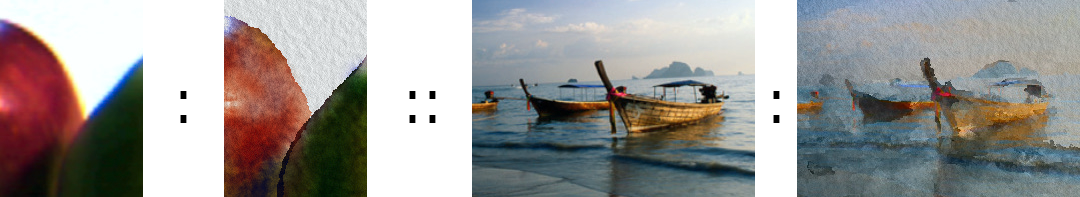
\includegraphics[width=\linewidth*2/3]{files/assets/articles/heartzmann1.png}
	\caption{...}
	\label{img:preview}
\end{figure}

\begin{figure}[!ht]
	\centering
	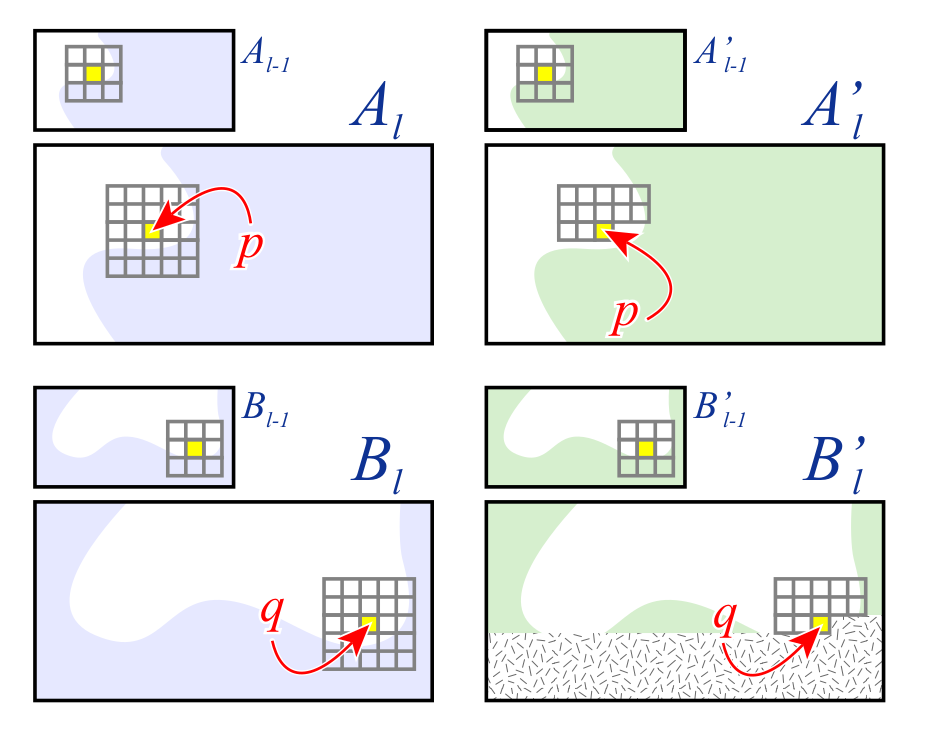
\includegraphics[width=\linewidth*2/3]{files/assets/articles/heartzmann2.png}
	\caption{...}
	\label{img:preview}
\end{figure}


\section{Transferência de estilo} 

O método de ``Style Transfer'' proposto
por Gatys, Ecker e Bethge \cite{Gatys2016}
nos permite, alem de re-amostrar a textura,
controlar a geometria do resultado.
Para isso o algoritmo recebe duas imagens,
uma definirá o estilo
e outra definirá o conteúdo do resultado.

...

\begin{figure}[!ht]
	\centering
	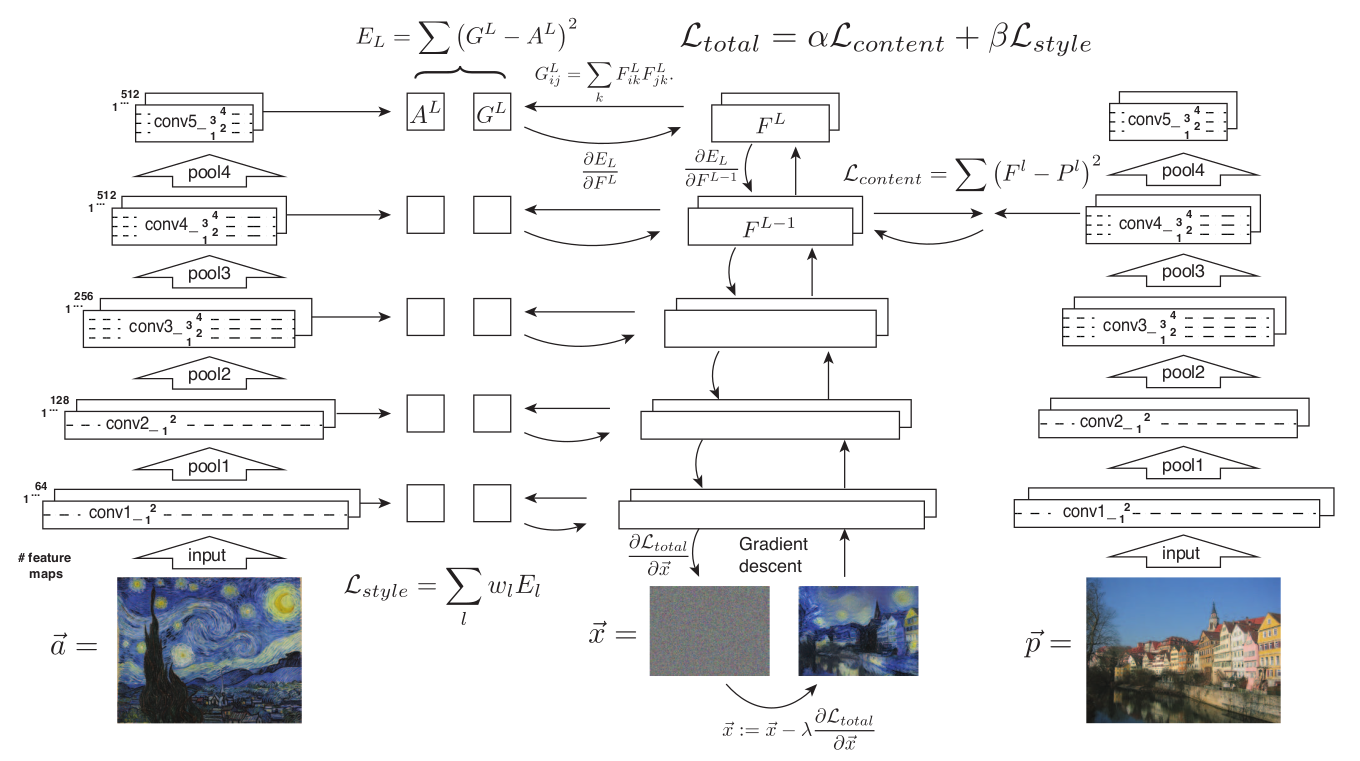
\includegraphics[width=\linewidth]{files/assets/articles/gatys3.png}
	\caption{...}
	\label{img:preview}
\end{figure}


% Definir e mostrar resultados

% Falar do deepart.io?

\fi